% LaTeX.tex
% Template for PROCEEDINGS PAPER of the 27th ABCM International Congress of Mechanical Engineering
% COBEM 2023
% Based on the templates of COBEM2015, COBEM2017, COBEM2019 and COBEM2021

\documentclass[10pt,fleqn,a4paper,twoside]{article}
\usepackage{abcm}
\usepackage{amssymb,amsmath,amsthm,fancyhdr,mathabx}
\usepackage{multirow}
\usepackage{subfig}

\def\shortauthor{F. Author, S. Author and T. Author (update this heading accordingly)}
\def\shorttitle{Rocket Nozzle Inverse Design Using a Machine Learning Flow Reconstruction Technique}

\begin{document}
\fphead
\hspace*{-2.5mm}\begin{tabular}{||p{\textwidth}}
\begin{center}
\vspace{-4mm}
\title{
DATA-DRIVEN FLOW RECONSTRUCTION USING LOW FIDELITY SIMULATION FOR COMPRESSIBLE FLOW PREDICTIONS IN CONVERGENT-DIVERGENT NOZZLES}

\end{center}
\authors{Allan Moreira de Carvalho} \\
\authors{Daniel Jonas Dezan} \\
\authors{Wallace Gusmão Ferreira} \\
\institution{Federal University of ABC, Santo André - SP, Brazil} \\
\institution{allan.carvalho@ufabc.edu.br} \\
\institution{daniel.dezan@ufabc.edu.br} \\
\institution{wallace.ferreira@ufabc.edu.br} \\ %(If all authors are from the same institution, the "Institution and address" must be placed only once.)
%\institution{e-mail} \\
\\
%\authors{Same format for other authors, if any} \\
\\
\abstract{\textbf{Abstract.} The rise in computing power has made numerical experiments more accessible and efficient for complex problems. Machine learning methods are seen as complementary to traditional methods in processing vast amounts of data. In the field of supersonic nozzle aerothermodynamics, predicting wall heat transfer is crucial. High-fidelity methods, such as RANS, are commonly used. This study implements a surrogate model using dimensional reduction and ANNs/Kriging to map low-fidelity results to the high-fidelity method. Results show that a quasi-1D Euler solver can accurately reconstruct a 2D viscous flow. A comparison of the Neural Network and Kriging methods showed comparable performance, with Kriging being faster and more accurate. The reduction method used POD effectively reduced the data to 10 latent variables with minimal loss of information.}\\
\\
\keywords{\textbf{Keywords:} Flow reconstruction, neural Networks, kriging, reduced order model.}\\
\end{tabular}

\section{INTRODUCTION}

Simulations are essential in many areas of science and engineering, and the more accurate the simulation, the better. However, the computational cost of these simulations can be quite high, especially when aiming for high accuracy. To mitigate this, various numerical methods have been developed, but they all come with a trade-off: the more accurate the method, the more computationally expensive it is. This can lead to results that are compromised by the available time and resources. A common solution to this problem is to use a simplified version of the original numerical method, such as using a coarse resolution or cutting out certain physical phenomena. However, this can have a significant impact on what can be inferred from the results, compromising final applications such as optimum design, control, and inverse problems.

The main objective of this work is to use model order reduction to compress data \citep{Hesthaven2016} and Neural Network\citep{Yu2019}/Kriging\citep{Ng2018}, acting as a universal nonlinear mapping from the reduced, simplified domain to the full model domain. The problem at hand is to find the heat flux and internal wall temperature for each boundary condition of the flow field of air over a convergent-divergent nozzle, with its walls cooled by water. This problem can be solved numerically by a conjugate heat transfer model, solving the Navier-Stokes equations for the fluid domain and the heat equation for the solid domain, in an iterative manner until the temperature at the fluid-solid interface converges. This is the full, or high-fidelity model.

A simplified model that solves for only one dimension and ignores viscosity is cheaper to calculate, but can't predict heat transfer on nozzle walls. This is known as the low-fidelity model. A reduced-order surrogate model combined with a Neural Network/Kringing can predict the full 2D flow field of the high-fidelity model with minimal increase in computation cost compared to the low-fidelity model.

The increasing interest in using neural networks as a machine learning method for fluid reconstruction has motivated this work \citep{Ozbay22,Ma2022,Dubois2022,Erichson2020}. The main objective is to compare the neural network approach with the established Kriging interpolation method.

The numerical methods used in both low and high-fidelity models are described, including verification and a study of grid independence. The study includes the presentation and comparison of two reduced-order models: one using a Neural Network and the other using Kriging. The comparison focuses on computation time and the accuracy of reconstruction, as determined by a testing dataset.

\section{METHODOLOGY}

\subsection{Low fidelity model}

The low-fidelity model in this work is a quasi-one-dimensional Euler solver that captures the main problem features while disregarding those only captured by the high-fidelity model. The model solves for the conservation of mass, momentum, and energy over a regular mesh, with simplifications such as an inviscid fluid with constant properties and constant cross-sectional areas of the nozzle. The model is unable to predict heat transfer at the walls as it only solves for the fluid domain. The numerical method used is an in-house finite volume solver for the conservative variables $\mathbf{U} = \left[ \rho \quad \rho u \quad e \right]^T$, using the conservation law in Eq.~(\ref{eq:q1deuler}) \citep{Babu2020}, where $\mathbf{F} = \left[ \rho u \quad \rho u^2 + p \quad (e+p)u \right]$ represents the inviscid flux, $S=S(x)$ represents the cross-sectional area, and $\mathbf{Q} = \left[ 0 \quad \frac{p}{S}\frac{dS}{dx} \quad 0 \right]$ represents the source term arising from dimensional shrink.

\begin{equation}
\frac{\partial \mathbf{U}}{\partial t}+\frac{1}{S} \frac{\partial(\mathbf{F} S)}{\partial x}=\mathbf{Q}
\label{eq:q1deuler}
\end{equation}

The system is based on the assumption of an ideal gas. The code "eulerQ1D" uses the finite volume method to solve equation Eq.~(\ref{eq:q1deuler}) and employs the Steger-Warming method for spatial discretization. It also uses the AUSM method to evaluate the fluxes. To achieve steady-state solution, time marching is utilized along with a fourth-order Runge-Kutta integrator.

\subsubsection{Verification}

The numerical method was verified by comparing its results to those presented in reference \citep{ARINA2004409}. The nozzle shape is defined by equation Eq.~(\ref{eq:arinanozzle}) and is located within the domain $0 < x < L$, with $xt = 5.0$.

\begin{equation}
S(x)= \begin{cases}2.5+3\left(\frac{x}{x_t}-1.5\right)\left(\frac{x}{x_t}\right)^2 & , \text { if } x \leqslant x_t \\ 3.5-\frac{x}{x_t}\left[6-4.5 \frac{x}{x_t}+\left(\frac{x}{x_t}\right)^2\right] & , \text { if } x>x_t\end{cases}
\label{eq:arinanozzle}
\end{equation}

\begin{figure}[!ht]
	\begin{center}
		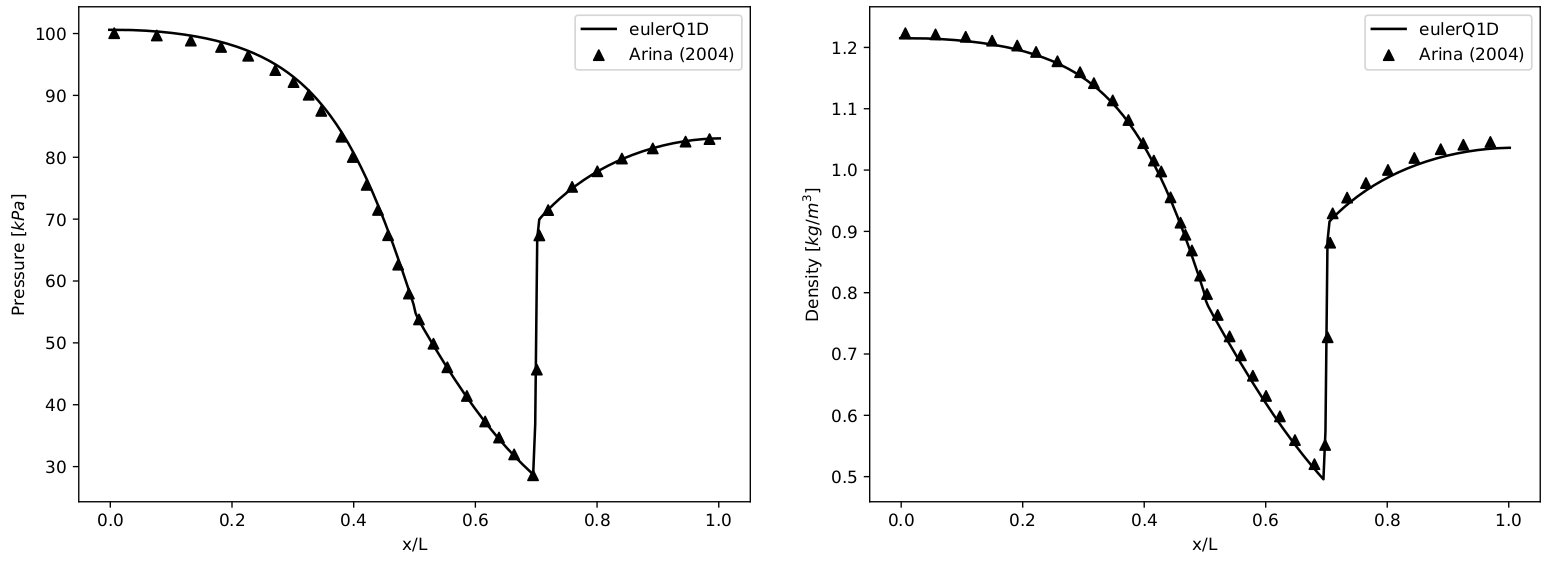
\includegraphics[width=\textwidth]{images/arina_validation.png}
		\caption{A comparison of the pressure (left) and density (right) profiles obtained through our in-house solver and the numerical results presented in \cite{ARINA2004409} is shown.}
        \label{fig:arina}
	\end{center}
\end{figure}

The input parameters for this study include a stagnation pressure of 104,074 kPa and a stagnation temperature of 291.3 K ant the inlet. The outlet boundary condition is defined as the static pressure of 83,049 kPa. The specific gas constant and ratio of specific heats for Air, as an ideal gas, are given as $R = 287$ J/kg/K and $\gamma = 1.4$, respectively. The results obtained in this work were compared to previously published data, as shown in Figure \ref{fig:arina} . The pressure and density profiles along the nozzle match the results presented by Arina, demonstrating that this method is effective in accurately capturing the position of the shock wave, which is represented by a discontinuity in Figure \ref{fig:arina}.

\subsection{High fidelity model}

The SU2 software \citep{Economon2016} was employed to address the conjugate heat transfer interfaces between the fluid and solid in the nozzle. In the fluid domain, the Reynolds Averaged Navier-Stokes equations were solved using the finite volume method and the SST (Shear Stress Transport) turbulence model. To obtain the steady-state solution, the implicit Euler integration method was utilized in conjunction with time marching. On the other hand, for the solid domain, the energy equation was solved.

\subsubsection{Verification - Grid Independence Study}

A Grid Independence Study using the Grid Convergence Index (GCI)\cite{roache1994} was performed to assess numerical accuracy. Table \ref{tab:meshesgci} lists the three mesh levels used and Table \ref{tab:gci} shows the results. Positive $\hat{p}$ and small GCI values indicate a monotonic and asymptotic convergence, respectively. A $GCI_{asymptotic}$ close to 1 indicates grid-independent solutions, so grid 2 was chosen for further analysis (shown in Figure \ref{fig:grid_selected}).

\begin{table} [ht]
	\caption{Numerical domains for grid independence study.}
    \label{tab:meshesgci}
	\begin{center}
		\begin{tabular}{@{}l|c|c|c|c|c@{}}        
            \hline
            & $N_x$ & $N_y$ & $ N_{cells} $ & $r$ & $Y^{+}$ \\ 
            \hline%\cline{1-5}
            Grid 1 & 160 & 250 & 118091 & 1.3 & $\approx 1$\\ 
            Grid 2 & 210 & 330  & 68761 & 1.3 & $\approx 2$\\ 
            Grid 3 & 270 & 440  & 39591 & -   & $\approx 3$\\
            \hline%
		\end{tabular}
	\end{center}
\end{table}

\begin{figure}[!ht]
	\begin{center}
		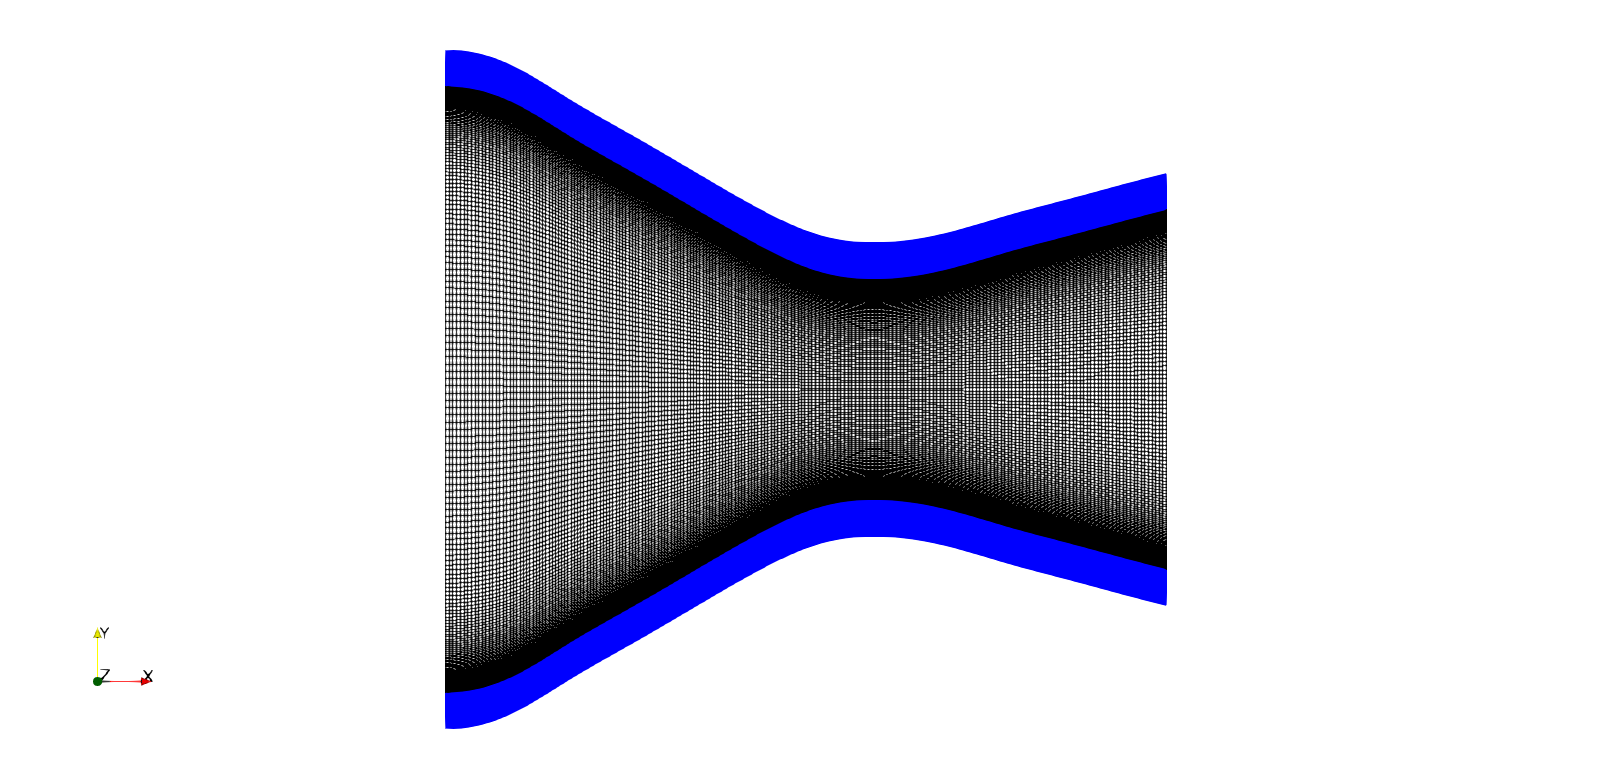
\includegraphics[width=\textwidth]{images/mesh.png}
        \caption{Grid 2, selected by the GCI analysis.}
        \label{fig:grid_selected}
	\end{center}
\end{figure}

\begin{table}
	\caption{Results for the grid independence study for average heat flux along the wall (q), pressure along center line (p) and temperature at the wall (T) of the nozzle.}
 \label{tab:gci}
	\begin{center}
		\begin{tabular}{@{}l|c|c|c|c|c|c|c@{}}
			\hline
& $ q \;[W/m^2] $ & $ N_{cells} $ & $ r $ & $ GCI $ & $ GCI_{asymptotic} $ & $ \hat{p} $ & $ q_{extrapolated} \;[W/m^2]$ \\ 
\hline%\cline{1-5}
Grid 1 & $519 \times 10^3$ & 118091 & 1.3 & 6.95\%   & \multirow{3}{*}{ 1.034 } & \multirow{3}{*}{ 1.71 } & \multirow{3}{*}{ $548 \times 10^3$ } \\ 
Grid 2 & $502 \times 10^3$ & 68761  & 1.3 & 11.40\% &                       &                      &                       \\ 
Grid 3 & $519 \times 10^3$ & 39591  & -   & -     &                       &                      &                       \\
\hline%

& $ p \;[kPa] $ & $ N_{cells} $ & $ r $ & $ GCI $ & $ GCI_{asymptotic} $ & $ \hat{p} $ & $ p_{extrapolated} \;[kPa]$ \\
\hline%\cline{1-5}
Grid 1 & $737 \times 10^3$ & 118091 & 1.3 & 0.23\%   & \multirow{3}{*}{ 1.001 } & \multirow{3}{*}{ 1.02 } & \multirow{3}{*}{ $738  \times 10^3$ } \\ 
Grid 2 & $736 \times 10^3$ & 68761  & 1.3 & 0.30\% &                       &                      &                       \\ 
Grid 3 & $736 \times 10^3$ & 39591  & -   & -     &                       &                      &                       \\
\hline%

 & $ T \;[K] $ & $ N_{cells} $ & $ r $ & $ GCI $ & $ GCI_{asymptotic} $ & $ \hat{p} $ & $ T_{extrapolated}\;[K] $ \\
\hline%\cline{1-5}
Grid 1 & $518$ & 118091 & 1.3 & 0.17\%   & \multirow{3}{*}{ 0.998 } & \multirow{3}{*}{ 3.73 } & \multirow{3}{*}{ $518$ } \\ 
Grid 2 & $520$ & 68761  & 1.3 & 0.47\% &                       &                      &                       \\ 
Grid 3 & $523$ & 39591  & -   & -     &                       &                      &                       \\
\hline%
		\end{tabular}
	\end{center}
\end{table}

\subsubsection{Validation}

Validating the high-fidelity model is difficult due to limited information on nozzle wall composition (assumed to be AISI 302). The test case used is test no. 313 from reference \cite{Back1964ConvectiveHT}. Boundary conditions were limited, with water temperature outside the wall set to a constant 300 K, causing slight deviation in temperature along the wall (Figure \ref{fig:validationtemperature}). However, the pressure distribution (Figure \ref{fig:validationpressure}) shows better agreement.

\begin{figure}[]
	\begin{center}
		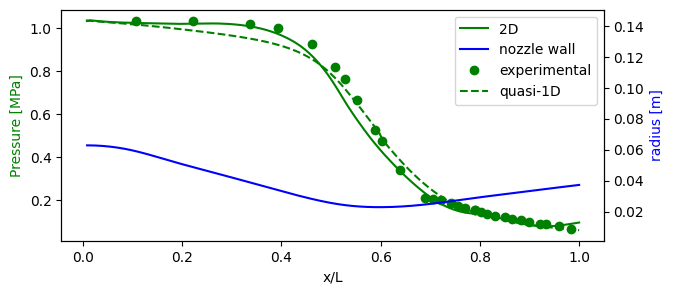
\includegraphics[]{images/validation_2d_2.png}
		\caption{Pressure distribution along nozzle centerline for for test. no. 313  \cite{Back1964ConvectiveHT} and numerical methods. }
        \label{fig:validationtemperature}
	\end{center} 
\end{figure}

\begin{figure}[]
	\begin{center}
		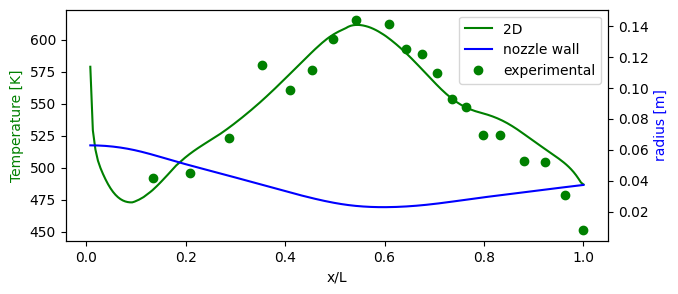
\includegraphics[]{images/validation_2d_1.png}
		\caption{Wall temperature distribution along the internal nozzle wall for experimental data from test. no. 313 \cite{Back1964ConvectiveHT} and numerical methods (this information can't be predicted by the quasi-one-dimensional model).}
        \label{fig:validationpressure}
	\end{center} 
\end{figure}


\section{REDUCED ORDER MODEL}

\subsection{Proper Ortoghonal Decomposition}

The Proper Orthogonal Decomposition (POD)\cite{Brunton2019} technique was used to reduce the dimension of both the low-fidelity and high-fidelity models, reducing thousands of degrees of freedom to a much smaller dimension. The snapshot for each i-th realization of the numerical models is a column vector filled with a desirable set of field variables. For the low-fidelity snapshot, $\chi_{l,i} = \left[ p \quad T \quad M\right]^T$ contains the pressure, temperature, and Mach fields. For the high-fidelity snapshots, $\chi_{h,i} = \left[ p \quad T \quad M \quad q_w\right]^T$, the pressure, temperature, Mach, and wall heat flux were selected.

To construct the snapshot matrices for equations \eqref{eq:snapshots}, we collected a set of 181 pairs of simulations by varying the inlet total temperature ($T_{0in}$) using latin hypercube sampling within the range of $285 < T_{0in} < 1115$ K.

\begin{align}
\mathbf{X_h} &= \left[ \chi_{l,0} \quad \chi_{l,1} \quad ... \quad \chi_{l,181}\right]^{208110 \times 181} \nonumber \\
\mathbf{X_l} &= \left[ \chi_{l,0} \quad \chi_{l,1} \quad ... \quad \chi_{l,181}\right]^{633 \times 181}
\label{eq:snapshots}
\end{align}

\subsubsection{Projection Error}

By utilizing the singular value decomposition with a rank of 10, we were able to accurately represent the dataset. Despite a significant reduction from 208110 to 10 degrees of freedom, the average global relative error in the Temperature field of 2D snapshots was as low as $0.0006$ \%. As shown in Figure \eqref{fig:projectionerror}, the maximum relative projection error for an arbitrarily chosen snapshot was negligible (0.0133 \%).

\begin{figure}[!ht]
	\begin{center}
		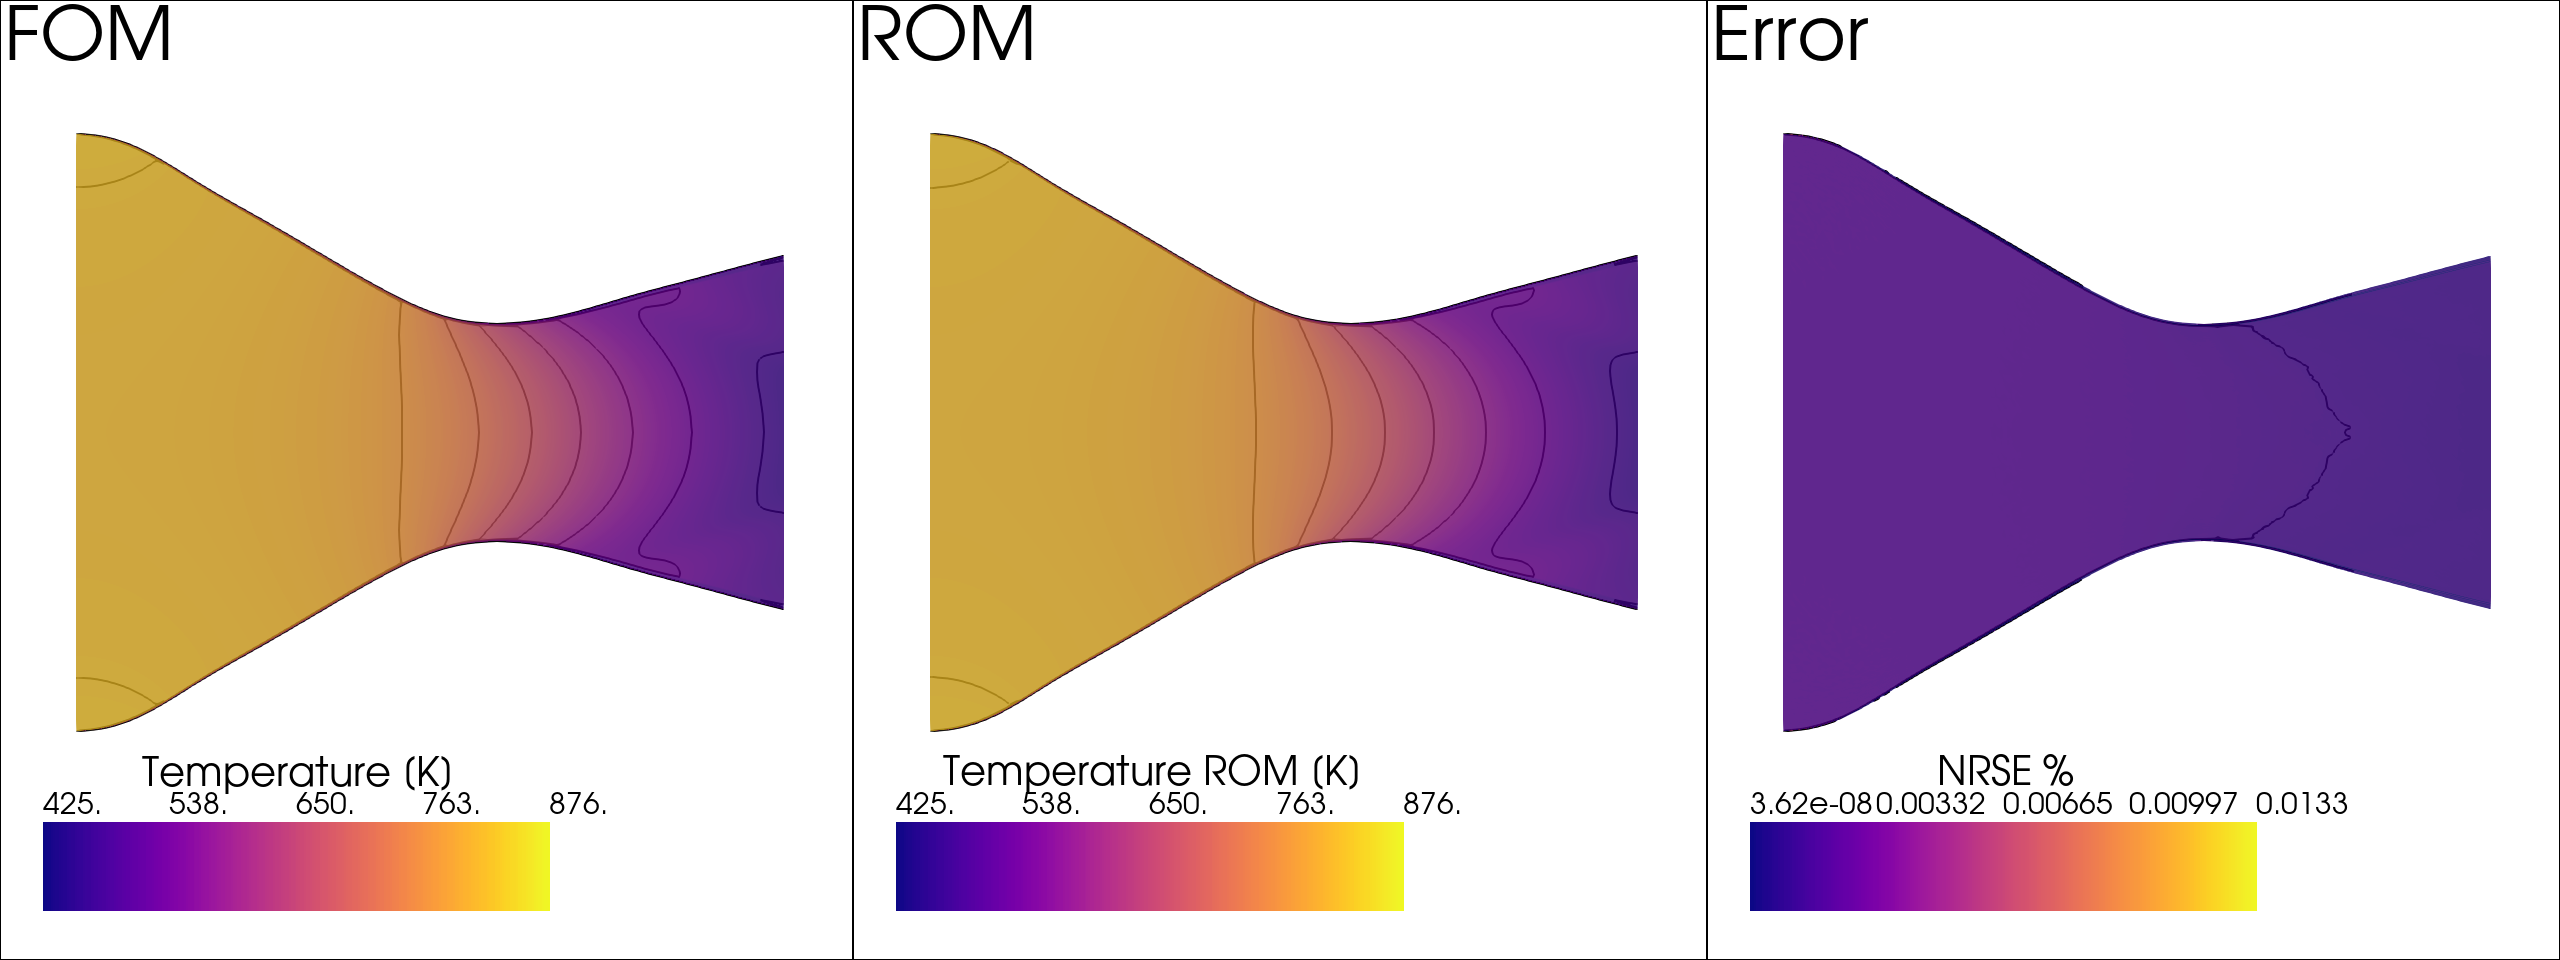
\includegraphics[width=\textwidth]{images/projection_error.png}
		\caption{The relative projection error for the temperature field for a simulation with an inlet temperature of 876 K, using 10 modes.}
        \label{fig:projectionerror}
	\end{center}  
\end{figure}

\subsection{Dense Neural Network}

In this work, a neural network (NN)\cite{Hornik1989} was used as a universal approximator to map the low-fidelity reduced space to the high-fidelity reduced space. The architecture of the NN is a dense multilayer perceptron built using the "tensorflow" library, with four layers of 10 neurons each. The activation function used was "tanh" and the optimizer was ADAM. Figure \ref{fig:history} illustrates the rapid decrease of the loss function, defined as the mean squared error between predictions and given data. Of the 181 pairs of snapshots, 145 were used to train the model, 18 were used for validation, and the remaining 18 were used for testing.

\begin{figure}[!ht]
	\begin{center}
		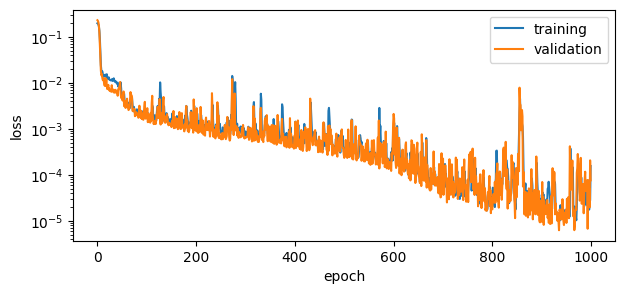
\includegraphics[width=\textwidth]{images/history.png}
		\caption{Neural Network training history.}
        \label{fig:history}
	\end{center}  
\end{figure}

\subsection{Kriging}

Kriging\cite{Forrester2008} is a continuous function interpolation method assuming a spatially correlated stochastic process. It minimizes prediction variance as the best linear unbiased predictor. This work applied ordinary kriging with exponential covariance model and no mean bias assumption. 145 snapshots from the 181-sample dataset were used for Kriging training, and the same 18-sample test dataset used for the neural network was used to test the Kriging model.

\section{Results}

The models were evaluated based on their ability to predict wall temperature and heat flux for a given nozzle flow with specified inlet stagnation temperature. The meta model algorithm is: (1) run a quasi-1D simulation with desired boundary conditions; (2) collect simulation results in a snapshot and project it into a pre-computed basis; (3) use the trained Neural Network/Kriging meta model to map reduced low-fidelity state to high-fidelity; (4) reconstruct the predicted high-fidelity embedding to the full state for analysis.

\subsection{Dense Neural Network}

Figure \ref{fig:onlinetest} demonstrates the quality of the obtained flow fields using a neural network as the metamodel, with a mean error for the Temperature field reconstruction of only 0.19 \%. Figure \ref{fig:onlinewall} illustrates the wall heat flux and wall temperature distribution predicted for the same test case, which are almost indistinguishable from the full-order model results.

\begin{figure}[!ht]
	\begin{center}
		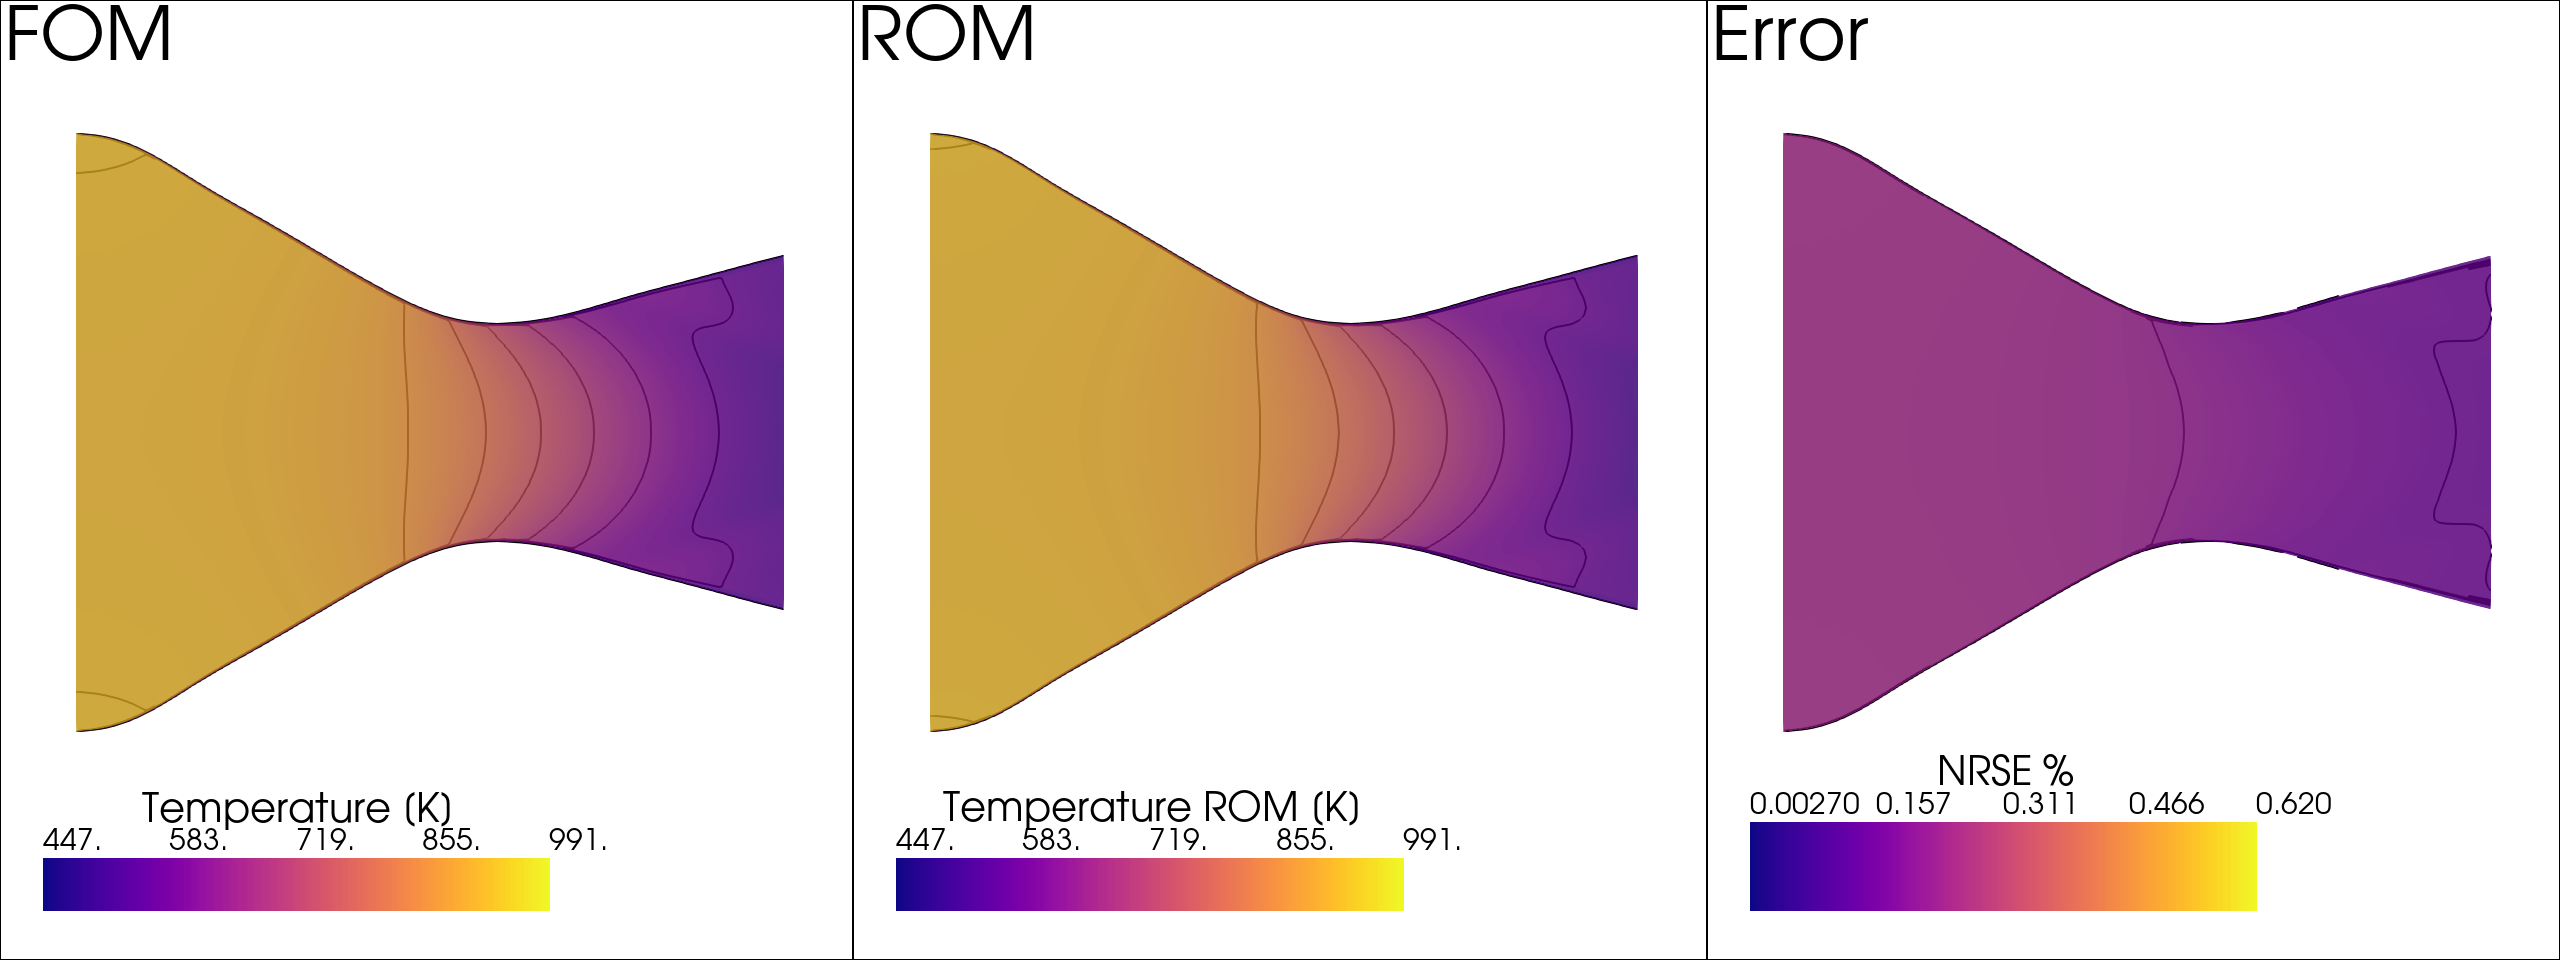
\includegraphics[width=\textwidth]{images/online_test_2d.png}
		\caption{Reconstruction result using a Neural Network to predict the temperature field for a test with inlet total temperature of $T_{0in}=935$ K.}
    \label{fig:onlinetest}
	\end{center}  
\end{figure}

\begin{figure}[!ht]%
    \centering
    \subfloat{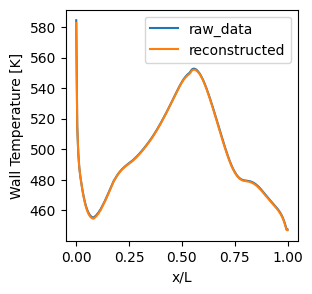
\includegraphics[width=0.45\textwidth]{images/online_Tw.png} }%
    \qquad
    \subfloat{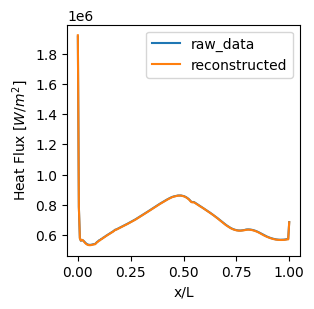
\includegraphics[width=0.45\textwidth]{images/online_q.png} }%
    \caption{Comparison of wall heat flux (right) and wall temperature (left) between the full-order model (raw\_data) and the results reconstructed by the reduced-order model (Neural Network method).}
    \label{fig:onlinewall}%
\end{figure}

\subsection{Kriging}

The Kriging method outperformed the Neural Network. Fig. \ref{fig:krigingtest} displays the normalized root mean squared reconstruction error for an arbitrary inlet total temperature boundary condition, which was $0.001\%$. The heat flux and wall temperature distributions were indistinguishable from the high-fidelity model, as shown in Fig. \ref{fig:krigingwall}.

\begin{figure}[!ht]
	\begin{center}
		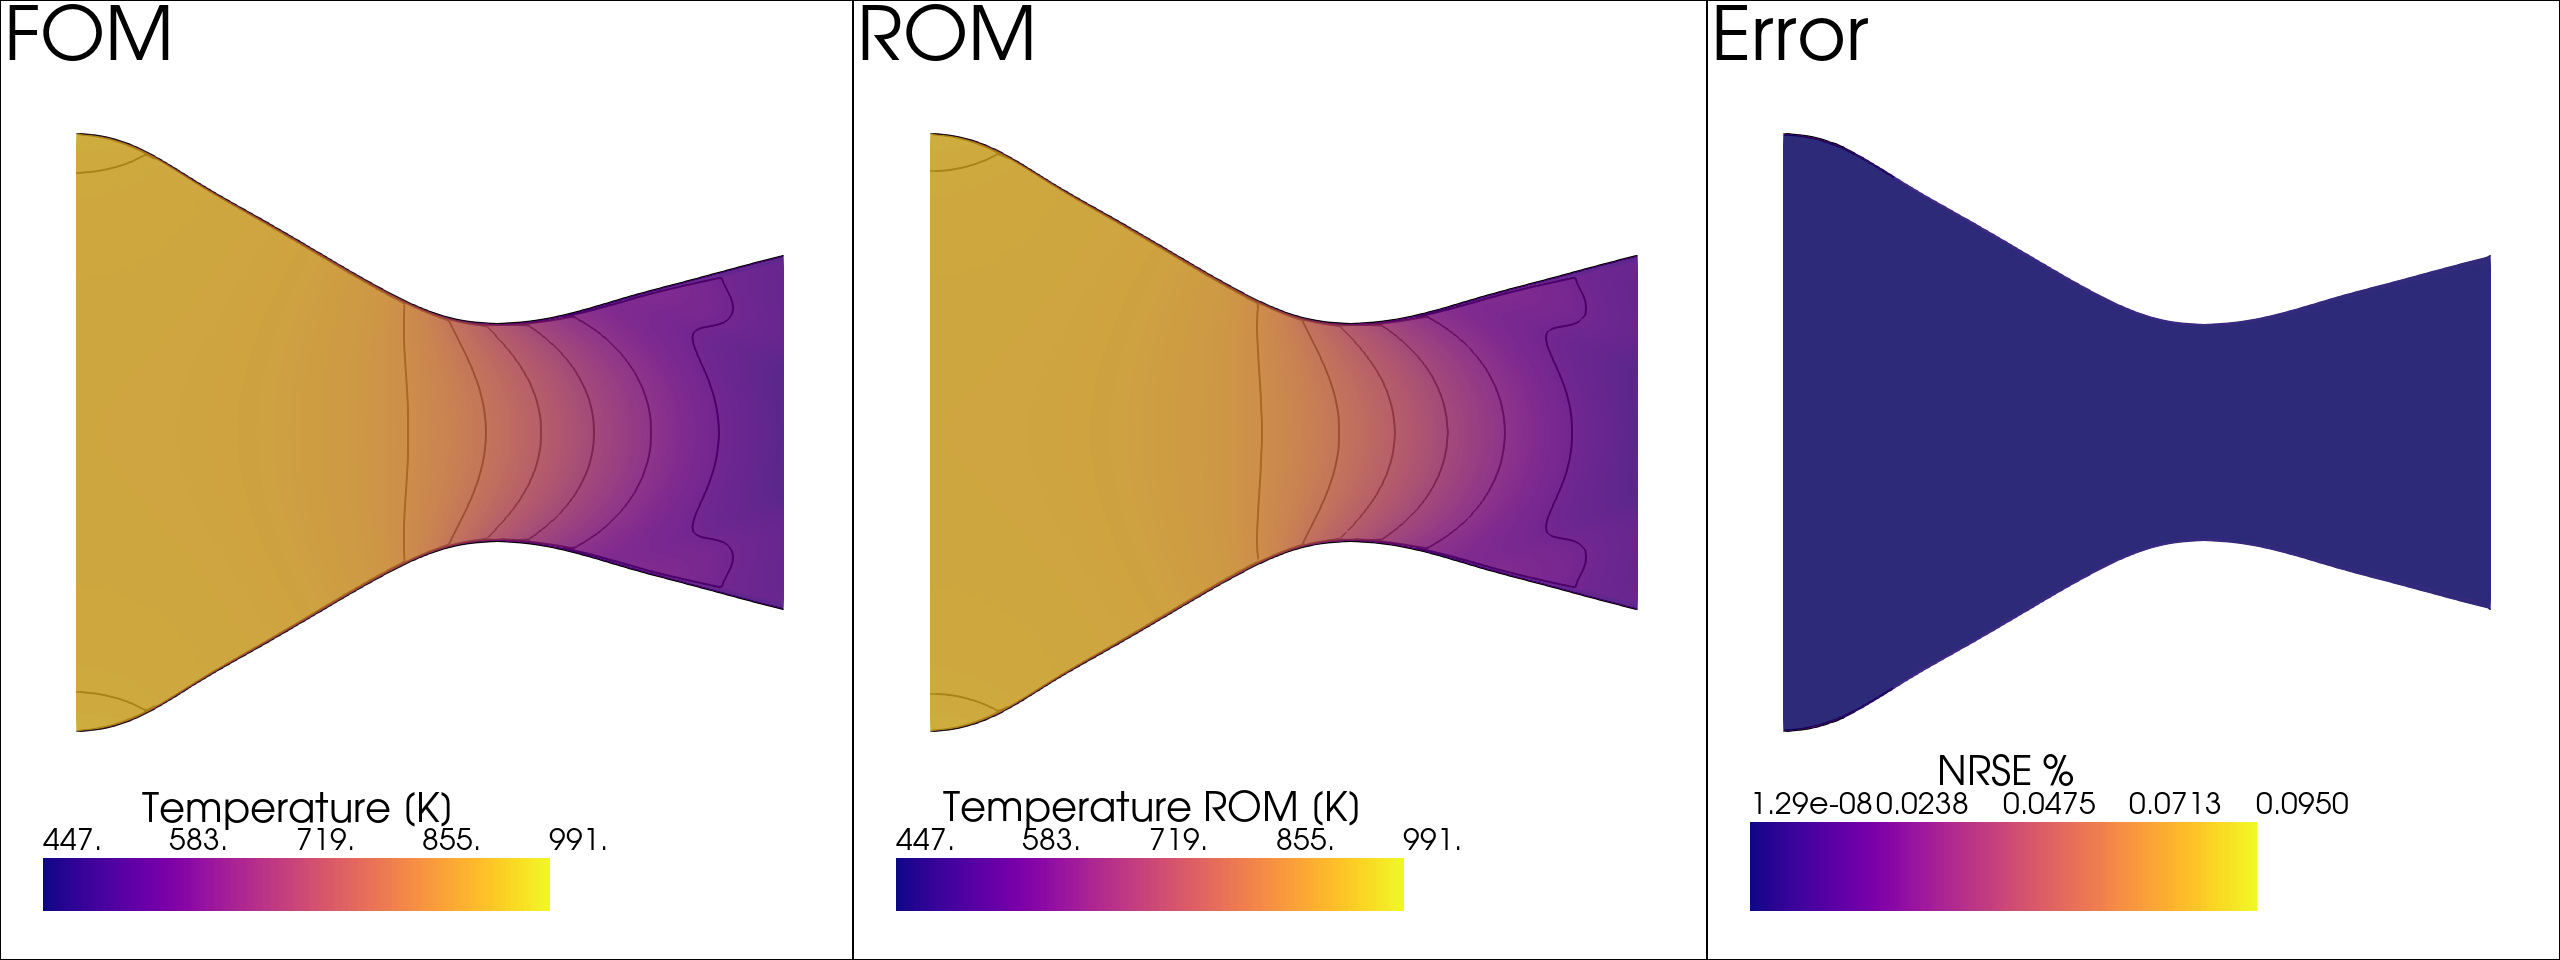
\includegraphics[width=\textwidth]{images/kriging_test_2d.png}
		\caption{Reconstruction result using Kriging to predict the temperature field of a test case with inlet total temperature of $T_{0in}=935$ K.}
    \label{fig:krigingtest}
	\end{center}  
\end{figure}

\begin{figure}[!ht]%
    \centering
    \subfloat{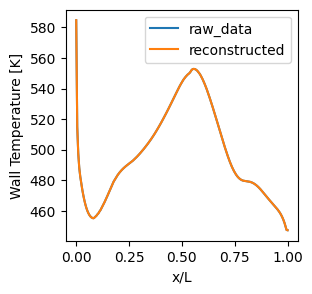
\includegraphics[width=0.45\textwidth]{images/kriging_Tw.png} }%
    \qquad
    \subfloat{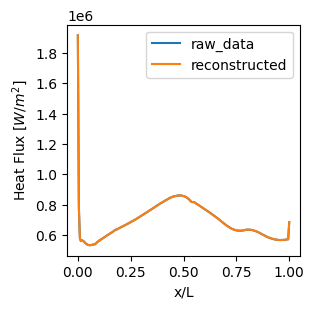
\includegraphics[width=0.45\textwidth]{images/kriging_q.png} }%
    \caption{Comparison of wall heat flux (right) and wall temperature (left) between the full-order model (raw\_data) and the results reconstructed by the reduced-order model (Kriging method).}
    \label{fig:krigingwall}%
\end{figure}

\subsection{Comparison}

The Reduced Order Model (ROM) offers a significant advantage in terms of evaluation time. Table \ref{tab:computcost} shows the relative speedup achieved. The Neural Network meta-model is more than 6,000 times faster than the full-order model, and the Kriging is over 38,000 times faster. Both models are highly accurate, with the greatest normalized mean squared error being less than 1.6% for the Neural Network and less than 0.05% for the Kriging.

\begin{table}  
	\caption{The computational cost of evaluating and training the model.}
     \label{tab:computcost}  
	\begin{center}
		\begin{tabular}{@{}l|c|c|c|c@{}}                 
            \hline%
            & CPU time & speedup & NRMSE - T & NRMSE - q \\ 
            \hline%\cline{1-5}
            high-fidelity model  & 1,532.42 seconds & - &  & \\
            low-fidelity model & 1.02 second & 1,502.37 $\times$ faster &  & \\ 
            NN training & 231.14 seconds & 6.63 $\times$ faster  &  & \\
            Kriging training & 1.63 seconds & 940.13 $\times$ faster  &  & \\
            single NN evaluation & 0.23 second  & 6,662.70 $\times$ faster & 1.38 \%  & 1.55 \% \\
            single Kriging evaluation & 0.04 second  & 38,310.50 $\times$ faster & 0.01 \%  & 0.04 \% \\
            full dataset computation & 271,587 seconds & 177.23 $\times$ slower &  & \\
            \hline%
		\end{tabular}
	\end{center}
\end{table}

\section{CONCLUSIONS}

This article describes a method for building Reduced Order Models (ROMs) to predict heat transfer in water-cooled nozzles. The procedure covers the essential elements of the numerical model, reduced order technique, and construction and training of the Neural Network/Kriging models. The code used in this study is available to the public.

Online testing showed that the ROMs are highly accurate, with a mean relative error of less than 1.6\%. This accuracy is particularly impressive given that the ROMs are nearly 40,000 times faster than full-order models. The ROMs have a wide range of applications, such as optimization, inverse design, control, and uncertainty quantification.

The study found that Kriging outperforms Neural Networks in terms of training cost, evaluation speed, and accuracy. This highlights the importance of considering mature interpolation techniques when building machine learning reduced order models for flow field analysis, rather than relying solely on modern neural network techniques.

\section{ACKNOWLEDGEMENTS}

The authors would like to thank IBM and CAPES/CNPq Brazilian agencies for the financial support to this work.


\section{REFERENCES} 
\label{Sec:references}

\bibliographystyle{abcm}
\renewcommand{\refname}{}
\bibliography{bibfile}


\end{document}
